\documentclass{article}
\usepackage[left=2cm,right=2cm,top=2cm,bottom=2cm]{geometry}
\usepackage[utf8]{inputenc}
\usepackage[german]{babel}
\usepackage{amsmath}
\usepackage{dsfont}
\usepackage[export]{adjustbox}
\usepackage{amsthm}
\usepackage{color}
\usepackage{amsfonts}
\usepackage{amssymb}
\usepackage{wasysym}
\usepackage{makeidx}
\usepackage{graphicx}
\usepackage[colorlinks=true,urlcolor=blue,linkcolor=blue]{hyperref}
\usepackage{ziffer}
\usepackage{minted}
\usepackage{xcolor}
\usepackage{framed}
\usepackage{mdframed}
\usepackage{subfiles}
\usemintedstyle{emacs}

\definecolor{purp}{HTML}{9A72AC}
\definecolor{re}{HTML}{FC6255}
\definecolor{gre}{HTML}{83C167}
\definecolor{blu}{HTML}{58C4DD}
\definecolor{shadecolor}{rgb}{0.85,0.85,0.85}
\definecolor{bg}{rgb}{0.95,0.95,0.95}
\setlength{\parindent}{0em} 

\BeforeBeginEnvironment{minted}{\begin{mdframed}[linewidth =2 ,backgroundcolor=bg , linecolor=black, linewidth=0.5]}
\AfterEndEnvironment{minted}{\end{mdframed}}

\newtheorem{defi}{Definition}
\BeforeBeginEnvironment{defi}{\begin{mdframed}[linewidth =2 ,backgroundcolor=bg , linecolor=black, linewidth=0.5]}
\AfterEndEnvironment{defi}{\end{mdframed}}

\newcommand{\bsp}{\textbf{Beispiel}:}
%\newcommand{\task}{\textbf{Aufgabe}:}

\newcommand{\bol}[1]{\textbf{#1}}
\newcommand{\q}[1]{\glqq #1\grqq}
\newcommand{\DODO}[1]{\textbf{\textcolor{red}{DODO:}} #1 \\ \begin{center}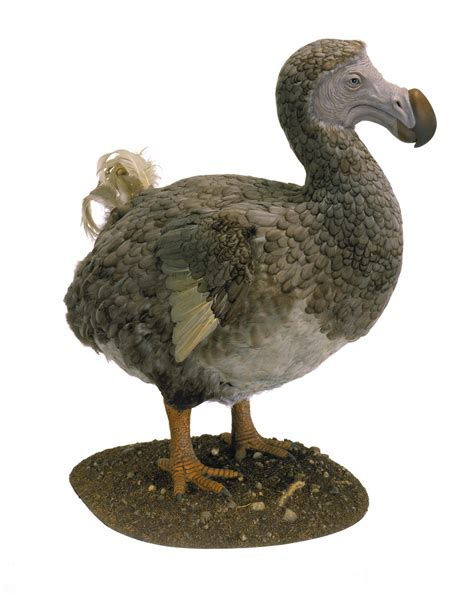
\includegraphics[scale=0.2]{../../media/dodo.jpg} \end{center}}

\newenvironment{task}[1]{
    \begin{shaded*}
    \textbf{Aufgabe #1}:
}{
    \end{shaded*}
}

\begin{document}
Die verkettete Liste erfüllt zwar alle Funktionalitäten, die wir von ihr erwarten, sieht man sich die Struktur aber genauer an, so erfüllt die Klasse Mensch eigentlich zwei Rollen. \\
\begin{center}
    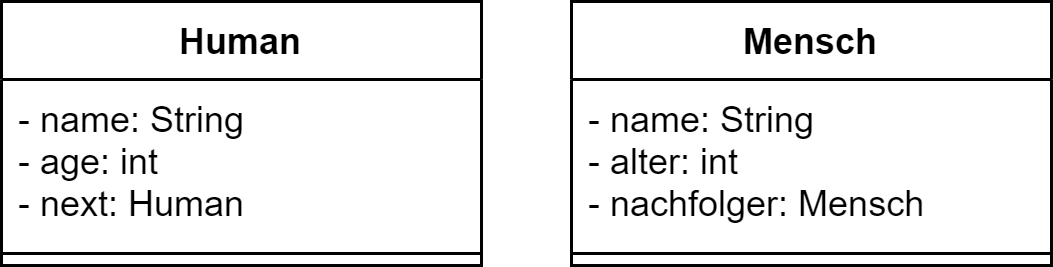
\includegraphics[scale = 0.2]{../media/human_v2.png}
\end{center}
Die ersten beiden Attribute beschreiben die eigentlichen Daten, die in dieser Liste gespeichert sind, dagegen ist das letzte Attribut für jemanden, der nur an den Menschen in der Schlange interessiert ist, irrelevant. \\
Das Problem wird noch deutlicher, nimmt man die Methoden hinzu: 
\begin{center}
    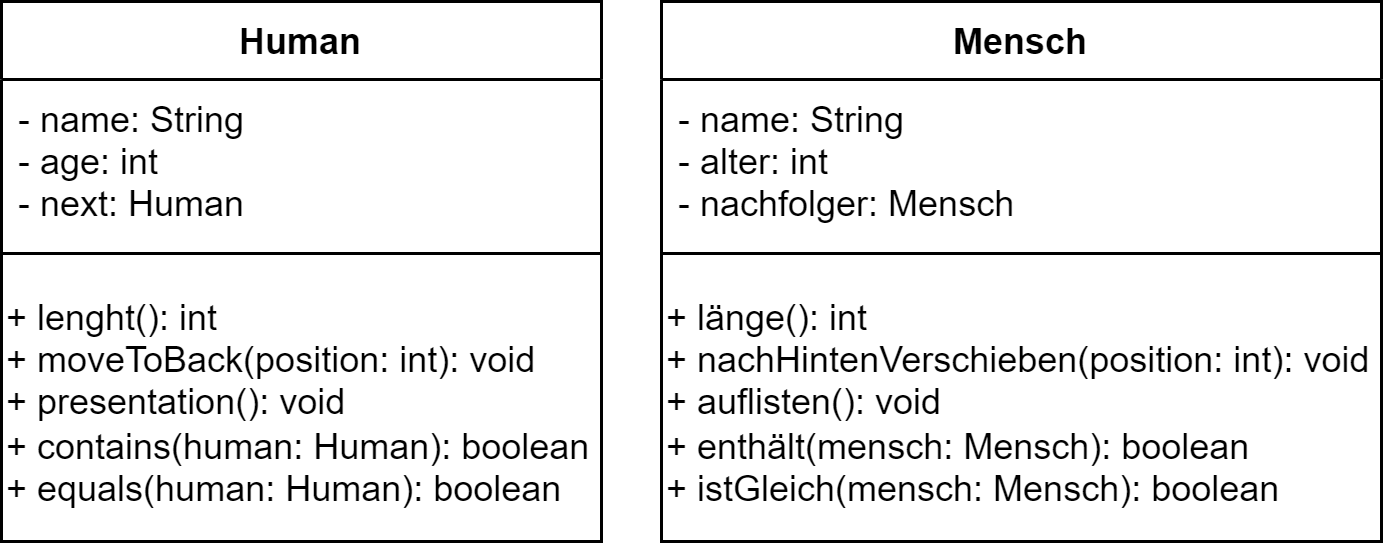
\includegraphics[scale = 0.2]{../media/human_v3.png}
\end{center}
Manche der Methoden sind nur notwendig, um die Liste zu durchlaufen und bestimmte Aktionen auszuführen - wie z.B. die Bestimmung der Länge. Welche Daten über den Menschen gespeichert sind, ist dabei völlig irrelevant. \\
Andere Methoden dagegen beziehen sich nur auf die Daten an sich, z.B. die istGleich(Mensch m) - Methode, die zwei Menschen miteinander vergleicht. \\
Diese Vermischung zweier unterschiedlicher sollte aufgelöst werden, d.h. eine Struktur geschaffen werden, die die Funktionalität der Liste enthält. In der Klasse Mensch verbleiben dann nur noch die Attribute und Methoden, die direkt mit den Daten zu tun haben. Auf diese Weise lässt sich die Liste auch leichter an neue Bedingungen anpassen. Wollen wir statt der Menschen eine Liste von Tieren anlegen, dann muss lediglich die Klasse Mensch und die Referenzen auf die Daten ausgetauscht werden. Die Liste an sich besteht dann aus ihrem \q{Kopf}, in unserem Fall die Warteschlange und mehrere Knoten. Jeder Knoten kennt dabei wieder seinen Nachfolger und hält eine Referenz zu einem Objekt der Klasse Mensch (in unserem Fall). Ohne detailliert auf die Methoden einzugehen sieht die Struktur also wie folgt aus: 
\begin{center}
    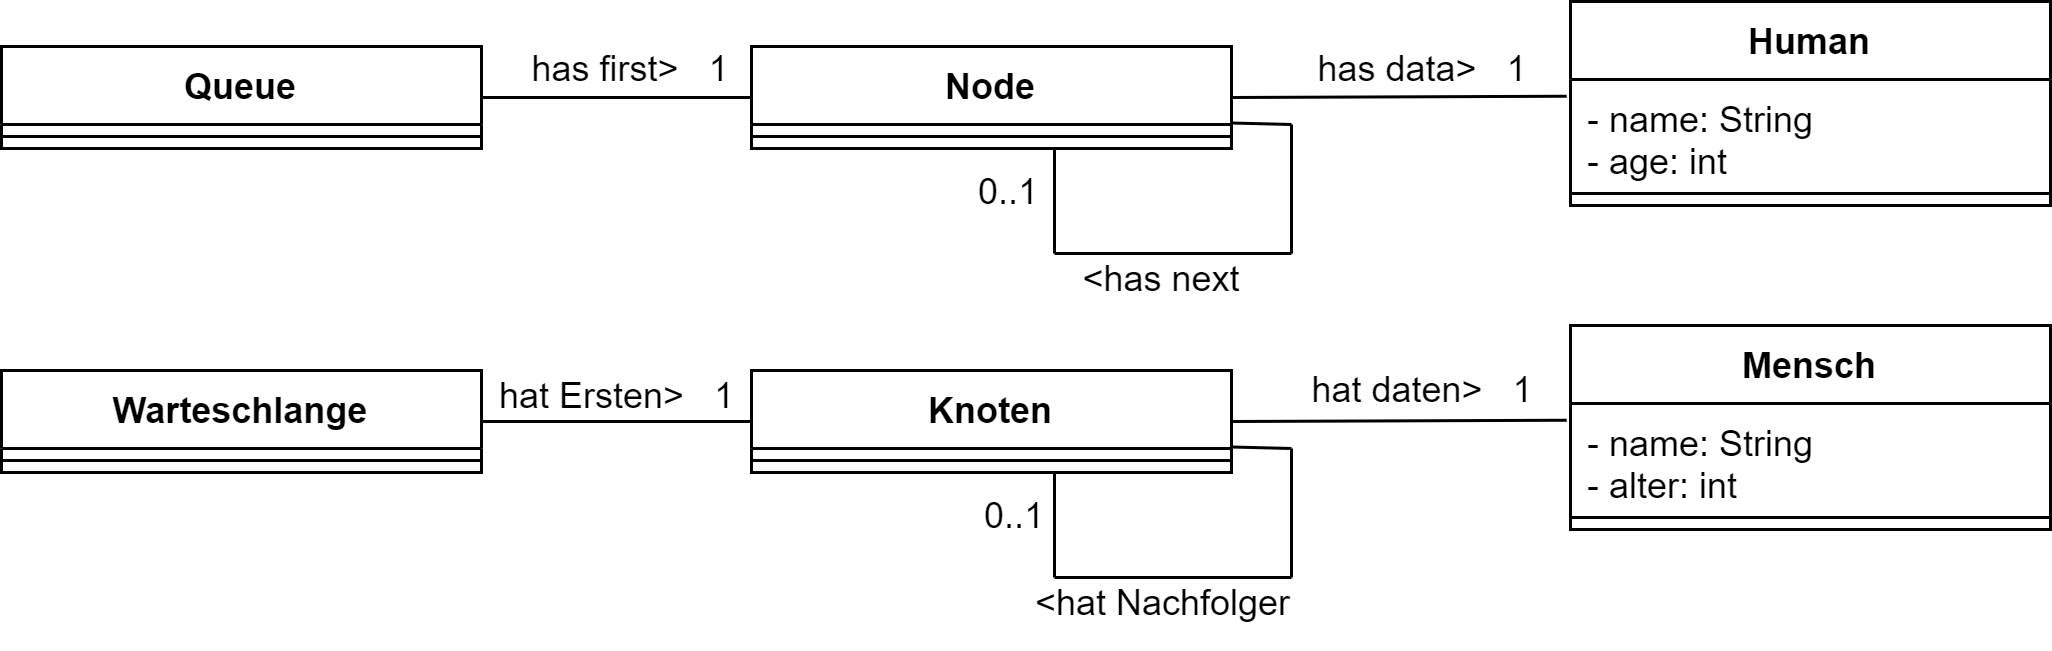
\includegraphics[scale = 0.2]{../media/linked_list_nodes_diagramm.png}
\end{center}
Die Klasse Knoten hat sich zwischen die Warteschlange und die \q{Datenklasse} Mensch geschoben. Alle Methoden, die wir bisher implementiert haben, lassen sich eindeutig einer der beiden Klassen zuordnen. In der Klasse Warteschlange ändert sich außer dem Namen der referenzierten Klasse bei keiner Methode etwas inhaltlich. \\
Angenommen wir betrachten eine Liste, die vier Menschen enthält, dann sähe ein Objektdiagramm der aktuellen Liste wie folgt aus: \\
\begin{center}
    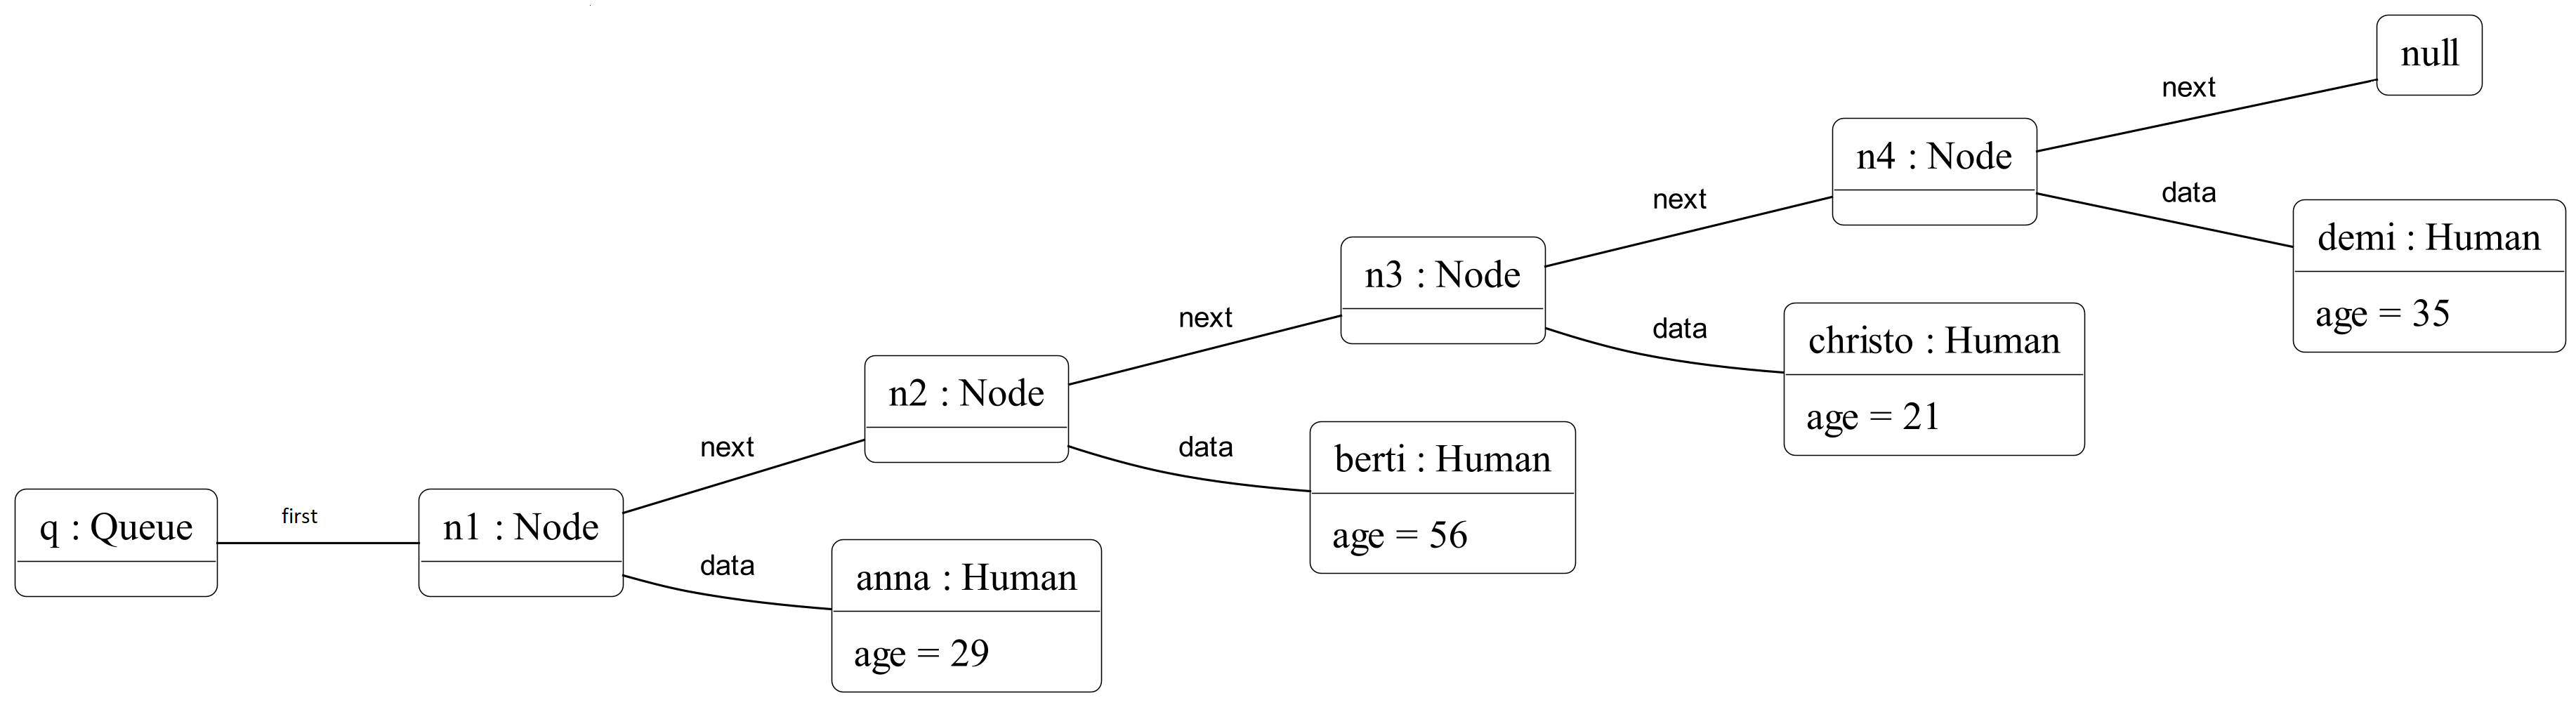
\includegraphics[scale = 0.14]{../media/linked_list_nodes_objectdiagram.png}
\end{center}
Das Gerüst der drei Klassen sieht dann wie folgt aus: 
\begin{minted}{Java}
    public class Queue {
        private Node human;

        public Queue() {
            human = null;
        }
    }

    public class Node {
        private Node next;
        private Human data;

        public Node(Human h) {
            next = null;
            data = h;
        }
    }

    public class Human {
        private int age;
        private String name;

        public Human(String name, int age) {
            this.name = name;
            this.age = age;
        }
    }
\end{minted}

\begin{task}{1}
    Implementieren Sie zur Übung die Methoden hintenEinfügen(Mensch m), vorneEntfernen() und auflisten() (bzw. push(Human h), pop() und printList()) für die neu definierte obige Struktur.
\end{task}

\vspace{2cm}

Wir könnten jetzt alle weiteren bisherigen Methoden auch für diese Modellierung implementieren. Es gibt jedoch vorher noch zwei Verbesserungen, die erste betrifft die Objekte, die wir an unsere Liste anhängen können. \\
Bisher können wir nur Elemente einer bestimmten Klasse an unsere Liste anhängen (dies entspricht auch den üblichen Implementierungen der von Java vorgegebenen Listentypen). Soll unsere Liste etwas flexibler werden - d.h., wir wollen Objekte verschiedener Klassen anhängen - so müssen wir sicherstellen, dass alle Klassen alle Methoden enthalten, die für die Liste notwendig sind. So muss beispielsweise jede Klasse eine istGleich() - Methode implementieren und die gespeicherten Daten auf Anfrage zurückgeben. \\
Um all dies zu realisieren bietet es sich an ein \textbf{Interface} zu verwenden. \\

\textbf{Einschub}: Interface \\
Neben einer (abstrakten) Oberklasse ist das Interface die zweite Möglichkeit in Java \q{allgemeines} Verhalten zu definieren. Im Interface werden nur Signaturen von Methoden definiert (und idealerweise kommentiert), eine Klasse die dieses Interface implementiert, muss dann diese Methoden überschreiben und mit konkretem Inhalt füllen. Ein einfaches Beispiel sind (mal wieder) Tiere. \\
\begin{minted}{Java}
    public interface AnimalMethods {
    /** 
    * Prints the typical sound of this animal onto the console.
    */
        public void animalSound();
    }

    public class Dog implements AnimalMethods {

        @Override 
        public void animalSound(){
            System.out.println("Woof!");
        }
    }

    public class Cat implements AnimalMethods {

        @Override 
        public void animalSound() {
            System.out.println("Meow!");
        }
    }
\end{minted}
Sowohl die Klasse Hund als auch die Klasse Katze implementieren das Interface und überschreiben die Methode geräuschMachen(). Es gibt dabei zwei große relevante Unterschiede zur abstrakten Klasse:
\begin{enumerate}
    \item Eine Klasse kann beliebig viele Interfaces implementieren, aber nur von einer Oberklasse erben. 
    \item Die Methoden müssen überschrieben werden und können nicht im Interface vordefiniert werden. Wird das Schlüsselwort \q{implements} verwendet erinnern gute IDEs auch daran mit dem Fehler: \q{The type $\cdots$ must implement the inherited abstract method $\cdots$}. Es sind also alle Methoden des Interface abstract, auch wenn das entsprechende Schlüsselwort nicht dabeisteht.
\end{enumerate}
\textit{Hinweis:} Die Anmerkung $@Override$ ist nicht zwingend nötig, wird aber von vielen IDEs automatisch erstellt, um deutlich zu machen, dass es sich um eine aus einer Oberklasse oder einem Interface überschriebene Methode handelt. \\
Zusammengefasst kann man sagen, dass mit einem Interface von einer Klasse eine bestimmte Funktionalität gefordert werden kann, ohne dass die Implementierungsdetails vorgegeben sind. \\
\textbf{Zurück zu unserem Anwendungsfall}: Wir wollen an unsere Liste nicht mehr nur Menschen anhängen, sondern alle Objekte von Klassen, die unseren Anforderungen an ein Datenelement genügen. Wir definieren also ein Interface Datenelement, in dem wir alle Methoden fordern, die wir benötigen. Wollen wir beispielsweise auch Tiere in unserer Warteschlange erlauben, so sähe die gewünschte Struktur so aus: 

\begin{center}
    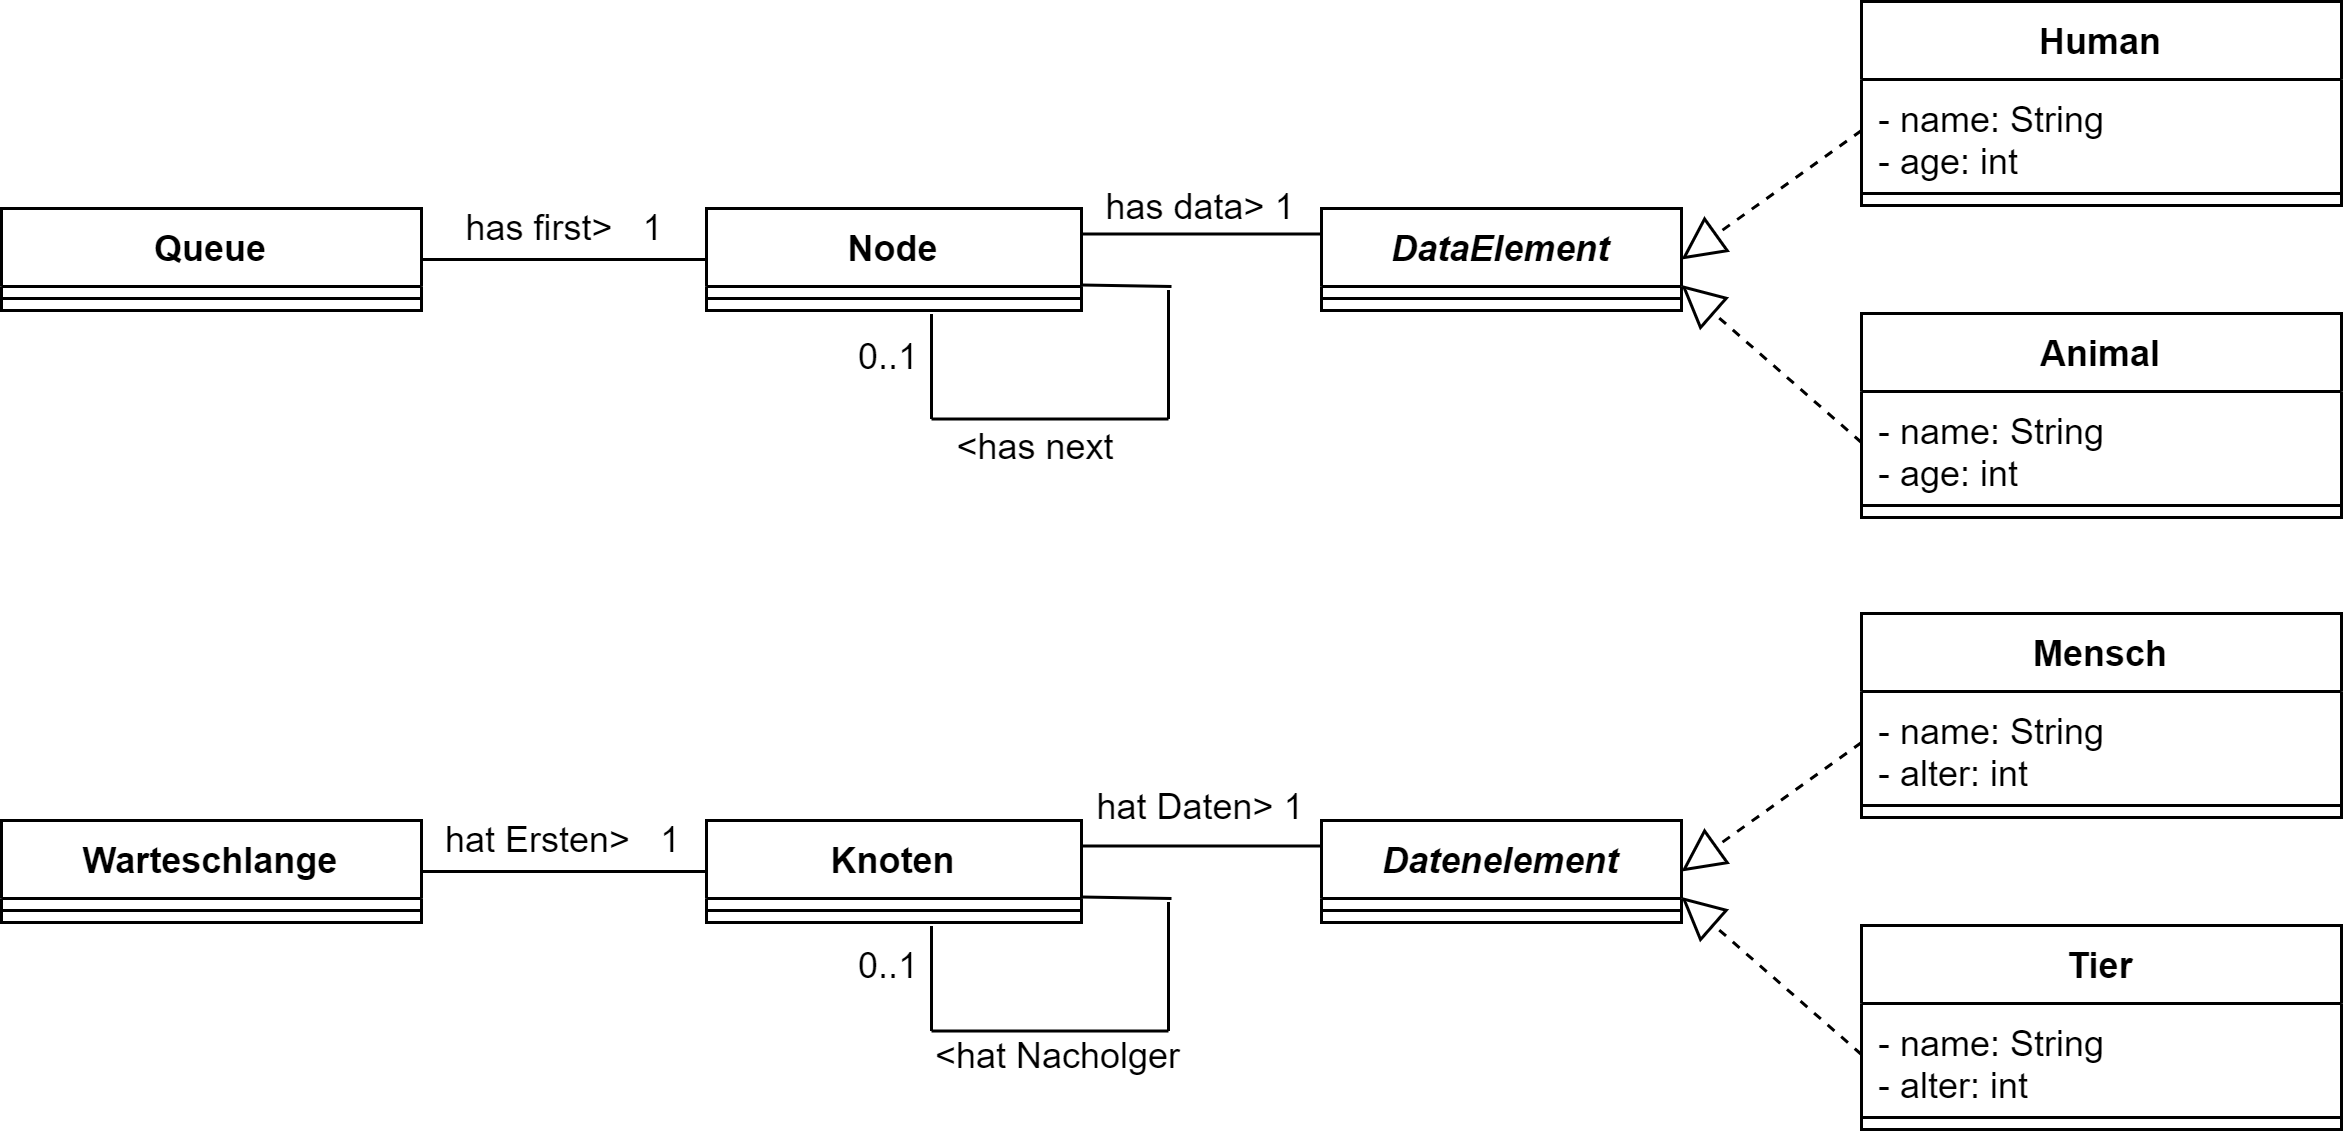
\includegraphics[scale = 0.2]{../media/linked_list_nodes_diagram_interface.png}
\end{center}
Betrachten wir die Warteschlange zu einem beliebign Zeitpunkt, dann ändert sich nicht viel: 

\begin{center}
    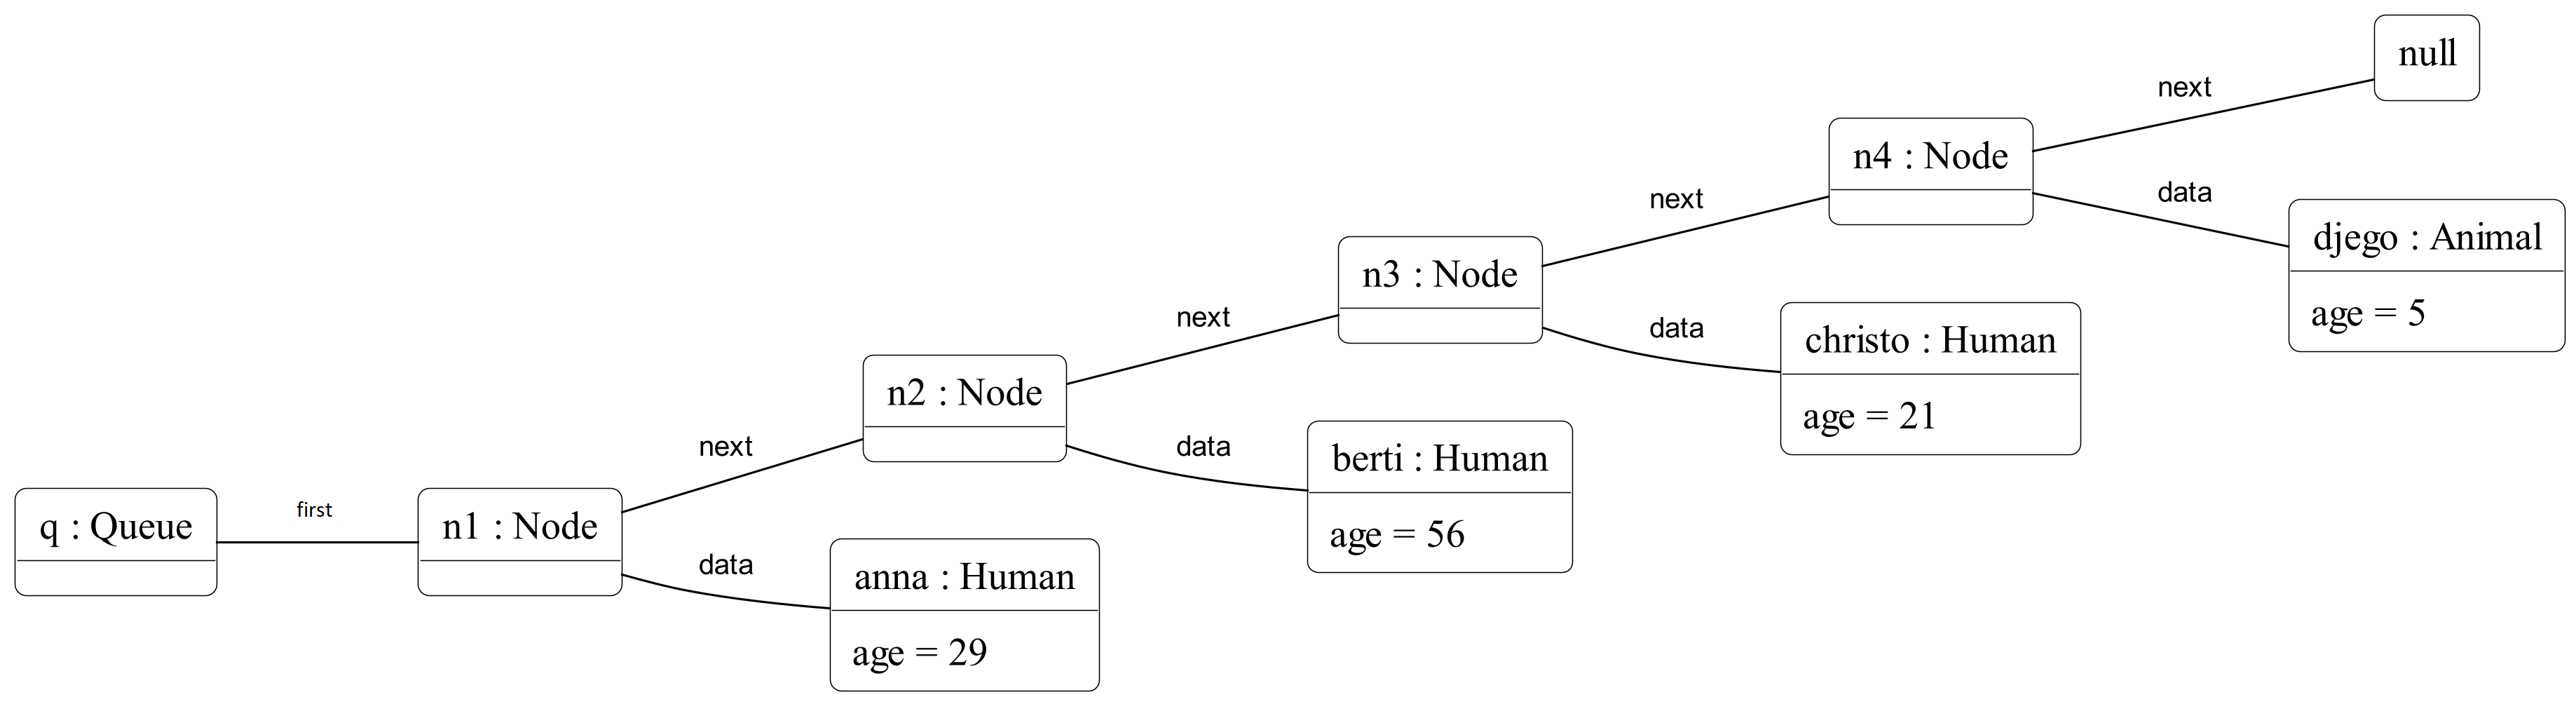
\includegraphics[scale = 0.125]{../media/linked_list_nodes_objectdiagram_v2.png}
\end{center}
Die grundlegende Struktur sieht dann wie folgt aus: 
\begin{minted}{Java}
    public class Queue {
        private Node human;

        public Queue() {
            human = null;
        }
    }

    public class Node {
        private Node next;
        private DataElement data;

        public Node(DataElement data) {
            next = null;
            this.data = data;
        }
    }

    public interface DataElement {
        ...
    }

    public class Human implements DataElement{
        private int age;
        private String name;

        public Human(String name, int age) {
            this.name = name;
            this.age = age;
        }
    }

    public class Animal implements DataElement{
        private int age;
        private String name;

        public Animal(String name, int age) {
            this.name = name;
            this.age = age;
        }     
    }
\end{minted}

\begin{task}{2}
    Implementieren Sie die Methoden hintenEinfügen(Mensch m), vorneEntfernen() und auflisten() (bzw. push(Human h), pop() und printList()) für die neu definierte obige Struktur. Beachten Sie dabei, dass in der Klasse Knoten auch ein Datenelement als Klasse gefordert werden kann, auch wenn es sich um ein Interface handelt. Letztendlich verlangt diese Syntax, dass in der Variable daten ein Objekt einer Klasse abgelegt wird, die das Interface Datenelement implementiert.
\end{task}

Im Folgenden finden sich die Lösungen für alle Methoden auf einmal, jeweils klassenweise dargestellt. Zuerst die derzeitige Warteschlange (die Bezeichner für die Liste werden inzwischen sehr lang, sollten mehrere Implementierungen im selben Java-Paket existieren ist diese Unterscheidung aber dringend notwendig!): 
\begin{minted}{Java}
    public class MyListLinkedNode {
        public MyListLinkedNode(){
            first = null;
        }

       public void push(DataElement data){
           Node node = new Node(data);
           if(first == null) {
               first = node;
           } else {
               first.push(node);
           }
       }

       @Override
       public DataElement pop(){
           if(first == null){
               return null;
           } else {
               DataElement toReturn = first.getData();
               first = first.getNext();
               return toReturn;
           }
       }

       @Override
       public void printList() {
           if(first == null){
               System.out.println("No list here to print!");
           } else {
               first.printList();
           }
       }
    }
\end{minted}
Die einzige Änderung zu den vorhergehenden Implementierungen sind die Ersetzungen der Klasse Mensch durch das Interface Datenelement und die Verwendung der gibDaten() Funktion, da die Daten nicht mehr direkt im Knotengespeichert sind, sondern dieser auch erst auf das Datenobjekt zugreifen müsste. In dieser Implementierung wird das gesamte Datenelement zurückgegeben, damit ggf. danach weiter damit gearbeitet werden kann. Möchte man noch mehr Kontrolle über die Daten haben, so könnte man im folgenden Interface ebenfalls eine String gibDaten() Funktion fordern, die die Daten im Element formatiert und als String zurückgibt.
\begin{minted}{Java}
    public interface DataElement {
        public void presentation();
    }
\end{minted}
Die Klasse Mensch verändert sich nicht wesentlich:
\begin{minted}{Java}
    
public class Human extends DataElement{
    private String name;
    private int age; 

    public Human(String name, int age){
        this.name = name;
        this.age = age;
    }

    @Override
    public void presentation(){
        System.out.println("I am " + name + " and I am " + age + " years old");
    }

    @Override
    public boolean equals(Object o){
        if(this == o) {
            return true;
        }
        if(! (o instanceof Human)){
            return false;
        } 
        Human h = (Human) o;
        if(h.getName() == this.name && h.getAge() == this.age){
            return true;
        } else {
            return false;
        }
    }
}
\end{minted}
Auf die getter- und setter-Methoden wurde aus Platzgründen verzichtet. \\
Es folgt die Klasse Knoten, die die rekursiven Aufrufe der Hauptklasse ausführt:
\begin{minted}{Java}
    public class Node {
        private Node next;
        private DataElement data;
        
        public Node(DataElement data){
            next = null;
            this.data = data;
        }

       public void setNext(Node node){
           next = node;
       }

       public Node getNext(){
           return next;
       }
   
        public void push(Node node){
            if(next == null){
                next = node;
            } else {
                next.push(node);
            }
        }

        public DataElement getData() {
            return data;
        }
  
        public void printList(){
            data.presentation();
            if (next != null) next.printList();
        }
    }
\end{minted}
Auch in dieser Klasse sind die Veränderungen überschaubar, lediglich an den Stellen, an denen mit den Daten interagiert wird hat sich die Syntax leicht verändert. \\
Betrachtet man die rekursiven Methoden, in diesem Fall die hintenAnfügen() und auflisten()-Methode, so wird noch eine \q{Schwäche} der Implementierung deutlich. Die Abbruchbedingungen der Rekursion sind mit einer Prüfung der Null-Referenz verknüpft. Diese Implementierung ist zwar nicht falsch, aber unelegant. Man kann diese Prüfungen vermeiden, indem man eine weitere Verbesserung vornimmt, die Verwendung eines Strukturmusters, des Kompositums. 

\begin{task}{4}
Zeichnen Sie ein vollständiges Klassendiagramm der obigen Implementierung. Ergänzen Sie außerdem die Klasse Tier und eine weitere selbst gewählte Klasse, die an die Liste angehängt werden kann. Fügen Sie bei den Methoden nicht nur die hinzu, die bereits implementiert sind, sondern greifen Sie auf Methoden aus vorherigen Kapiteln zurück und passen Sie deren Signaturen entsprechend der neuen Situation an. 
\end{task}
\end{document}